\begin{sepframe}{Complexity}
    {\scriptsize{Simplicity is the ultimate sophistication. L. Da Vinci}}
\end{sepframe}

\begin{frame}
    \frametitle{Complexity}
    \framesubtitle{Types}

    \begin{itemize}[<+->]
        \item Time complexity
        \item Space complexity
        \item Kolmogorov complexity
        \item Cyclomatic complexity
    \end{itemize}
\end{frame}

\begin{frame}
    \frametitle{Complexity}
    \framesubtitle{Time complexity}
    \lstinputlisting{src/session/complexity/resources/time-complexity-constant.php}
\end{frame}

\begin{frame}
    \frametitle{Complexity}
    \framesubtitle{Time complexity}
    \lstinputlisting{src/session/complexity/resources/time-complexity-linear.php}
\end{frame}

\begin{frame}
    \frametitle{Complexity}
    \framesubtitle{Time complexity}
    \lstinputlisting{src/session/complexity/resources/time-complexity-linear-alt.php}
\end{frame}

\begin{frame}
    \frametitle{Complexity}
    \framesubtitle{Time complexity}
    \lstinputlisting{src/session/complexity/resources/time-complexity-exp.php}
\end{frame}

\begin{frame}
    \frametitle{Complexity}
    \framesubtitle{Space complexity}
    \lstinputlisting{src/session/complexity/resources/space-complexity.php}
\end{frame}

\begin{frame}
    \frametitle{Complexity}
    \framesubtitle{Kolmogorov complexity}

    The Kolmogorov complexity is the shortest size of a program that yield the
    expected output.
\end{frame}

\begin{frame}
    \frametitle{Complexity}
    \framesubtitle{Kolmogorov complexity}

    Given the following outputs:

    \begin{itemize}[<+->]
        \item \texttt{1111111111111111111111111111111111111111}
        \item \texttt{0a05a9e69e5757ac71c75a50418622624f042c97}
    \end{itemize}
\end{frame}

\begin{frame}
    \frametitle{Complexity}
    \framesubtitle{Kolmogorov complexity}

    \lstinputlisting{src/session/complexity/resources/kolmogorov-complexity-example1.php}
\end{frame}

\begin{frame}
    \frametitle{Complexity}
    \framesubtitle{Kolmogorov complexity}

    \lstinputlisting{src/session/complexity/resources/kolmogorov-complexity-example2.php}
\end{frame}

\begin{frame}
    \frametitle{Complexity}
    \framesubtitle{Kolmogorov complexity}

    The Kolmogorov complexity is the generalization of Shannon's theory of
    information.
    \\
    It also has links to many other fields like with Gödel's incompleteness
    theorem, Turing's halting problem, compression theory, ...
    \\
    \bigskip
     \pause
    ``\textit{There is no way to tell if the K complexity of an algorithm is the
    shortest one}''.
\end{frame}

\begin{frame}
    \frametitle{Complexity}
    \framesubtitle{Cyclomatic complexity}

    \lstinputlisting{src/session/introduction/resources/complexity-example.php}
\end{frame}

\begin{frame}[fragile,c]
    \frametitle{Complexity}
    \framesubtitle{Cyclomatic complexity}

    \makebox[\linewidth]{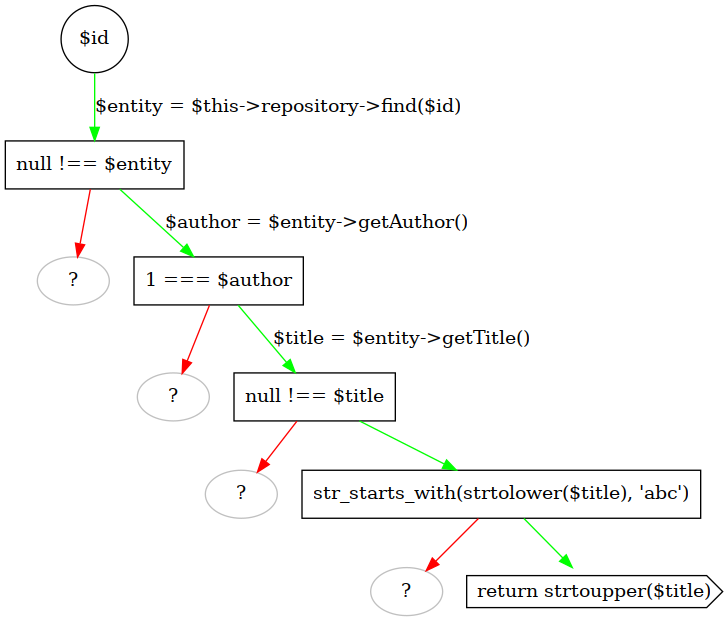
\includegraphics[height=.70\paperheight]{src/session/complexity/resources/complexity-example.png}}
\end{frame}

\begin{frame}[fragile,c]
    \frametitle{Complexity}
    \framesubtitle{Cyclomatic complexity}

    Conditions and type checks adds unnecessary complexity to a program,
    we are going to see how we can get rid of them.
\end{frame}

\begin{frame}[fragile,c]
    \frametitle{Complexity}
    \framesubtitle{Reducing the amount of nested conditions}

    But\pause\ but\pause\ but\pause ... we need conditions !
    \pause
    Of course.
\end{frame}

\begin{frame}[fragile,c]
    \frametitle{Complexity}
    \framesubtitle{Reducing the amount of nested conditions}

    EARLY RETURNS !
\end{frame}

\begin{frame}[fragile,c]
    \frametitle{Complexity}
    \framesubtitle{Cyclomatic complexity}

    \begin{lstlisting}[language=php]
    if ($expr1 && $expr2 && $expr3) {
        return true;
    }

    return false;
    \end{lstlisting}

    \pause

    is equivalent to:

    \begin{lstlisting}[language=php]
    if (! $expr1) {
        return false;
    }

    if (! $expr2) {
        return false;
    }

    if (! $expr3) {
        return false;
    }

    return true;
    \end{lstlisting}
\end{frame}


\begin{frame}
    \frametitle{Complexity}
    \framesubtitle{Cyclomatic complexity}

    \lstinputlisting{src/session/complexity/resources/complexity-example-early-returns.php}
\end{frame}

\begin{frame}
    \frametitle{Complexity}
    \framesubtitle{Cyclomatic complexity}

    \begin{itemize}[<+->]
        \item Think to the ``\textcolor{red}{unhappy}'' paths at first
        \item The ``\textcolor{green}{happy}'' path, is usually the last line,
        \item Easier to read, understand,
        \item Longer to write.
    \end{itemize}
\end{frame}

